%%=============================================================================
%% demo.tex for Xiamen University Graduate Thesis
%% modified by Maozhong Fu
%% Version: 1.0
%% Last update: 2020/09/30
%% Based on BIT-thesis at https://github.com/BIT-thesis/LaTeX-template
%%==============================================================================

% 默认单面打印 oneside 、硕士论文模板 master

\documentclass[twoside, pdf]{xmu-thesis-grd}

% 模板选项: 硕士论文 master; 博士论文 doctor; 直接使用学校doc文档转换的pdf页面 pdf

% 导入缩写词表
\input{chapters/acronym_list}

% 导入缩写词表
\input{chapters/symbol_list}

\begin{document}

%%%%%%%%%%%%%%%%%%%%%%%%%%%%%%
%% 封面及其他固定内容的页面
%%%%%%%%%%%%%%%%%%%%%%%%%%%%%%

% 中文封面内容,如果使用了pdf选项则这些不需要设置
% \title{资产重组:一个资不抵债国有企业的最佳选择}
% \author{某某某}
% \advisor{某某某教授}
% \major{信息与信号处理}
% \submitdate{2021年6月}
% \defenddate{2021年6月}
% \grantdate{2021年6月}
% \printdate{2021年6月}
%\studentnumber{**********}

% 封面
\makecover

% 学位论文原创性声明
\makeoriginalitystatement

% 学位论文著作权使用声明
\makecopyrightstatement

% 学位论文答辩委员会名单
\makenamelist

%%%%%%%%%%%%%%%%%%%%%%%%%%%%%%
%% 前置部分
%%%%%%%%%%%%%%%%%%%%%%%%%%%%%%
\frontmatter

% 中英文摘要
\input{chapters/abstract}

% 中英文目录
\tableofcontents
\entableofcontents

% 缩略词表
\makeacronymlist

% 符号表
\makesymbollist

% 图索引
\makefigurelist

% 表索引
\maketablelist

%%%%%%%%%%%%%%%%%%%%%%%%%%%%%%
%% 正文主体部分
%%%%%%%%%%%%%%%%%%%%%%%%%%%%%%
\mainmatter

%%==================================================
%% chapter01.tex for BIT Master Thesis
%% modified by yang yating
%% version: 0.1
%% last update: Dec 25th, 2016
%%==================================================
\chapter{绪论}
\enchapter{Introduction}
\label{chap:intro}
\section{研究意义及问题}
\ensection{Research Significance and Problems}

医学图像获取依赖于多种成像技术,包括计算机断层扫描(CT)\supercite{Ludwig2008,JournalNucMedTech2023}、磁共振成像(MRI)、放射性核素扫描和超声波等。这些技术各自揭示了生物组织的独特特征和信息,但也增加了图像的复杂性和多样性。CT成像基于X射线,通过捕捉不同组织对X射线的吸收差异来生成图像。与此相比,MRI利用磁场和无损耗的非离子辐射,对组织中的水分和脂肪进行成像,展现不同的组织特性。这些多样的成像方法提供了不同视角的生物组织图像,有助于更全面地了解人体内部结构和状况。医学图像分割是一项关键任务,旨在从整体医学图像中精确提取和标记出特定的结构或区域。这包括对器官、病变、血管等目标的识别和界定。这一过程对于深入理解和分析医学图像至关重要,它为医学研究、疾病诊断和治疗规划提供了关键支持。医学图像分割在定量分析和计算机辅助诊断系统中扮演着核心角色,使得对复杂医学图像的解读更加精确和高效。然而医学图像分割的数据标注过程通常需要耗费大量的人力和时间,且标注结果的质量和准确性往往受到标注者的经验和主观因素的影响。此外,医学图像的数据通常涉及隐私和安全问题,这也使得数据的共享和使用受到了严格的限制。因此,如何利用有限的标注数据并且保护数据隐私的情况下,实现医学图像分割的高效和精确成为了一个重要的研究问题。

为了在医学图像分割任务中提高效果并保护隐私,联邦学习提供了一种创新的解决方案。这种分布式学习方法的核心优势在于它允许多个数据持有者在不共享数据的前提下共同训练模型。虽然联邦学习一定程度上缓解了数据不足的问题,但在面对标注数据不足的挑战时,还可以采用自监督学习、半监督学习和迁移学习等策略。结合联邦学习和这些学习策略的应用,不仅能有效利用有限的标注数据提升模型性能,这还与OpenAI提出的模型scaling laws相契合,因为根据这些定律,大规模预训练模型往往需要大量的数据,而为大量数据进行标注在实际操作中并不可行。因此,这种结合联邦学习和以上各种学习策略的方法已成为实现医学图像分割的高效、精确且成本效益高的重要途径。

然而,该方向上仍存在以下亟待研究的关键问题:
* 在模型规模日趋庞大的情况下,之前的联邦学习框架都不能实现大规模模型的高效训练。这是因为联邦学习的核心特点是在不共享数据的前提下进行模型训练,这就意味着在联邦学习框架下,模型的训练数据是分布在多个数据持有者的设备上的,而这些设备的计算能力和存储能力往往是有限的。因此,如何在这种情况下实现高效的模型训练是一个重要的研究问题。
* 由于未标注数据和标注数据,不同的联邦学习参与者的数据分布往往是不同的,对模型性能有着不同程度的损害。如何消除这些非独立同分布的数据对模型训练的影响也是一个重要的研究问题。
* scaling laws在大量的其他领域被验证是正确的,如何利用这一规律来指导医学图像分割模型的训练是一个重要的研究问题。因为对于医学图像分割这一领域而言,对于精度的要求往往是非常高的,因此扩大模型的规模来获得更好的性能受益是非常有意义的。


\section{国内外研究现状}
\ensection{Research Progress Overview in Home and Abroad}


% \label{intro}

传统的集中式学习要求将在本地设备(如手机)上收集的所有数据集中存储在数据中心或云服务器上。这一要求不仅提出了隐私风险和数据泄露的担忧,而且当数据量巨大时,对服务器的存储和计算能力提出了高要求。尽管分布式数据并行\supercite{dean2012large},它允许多台机器并行训练具有不同数据组的模型副本,可能作为解决存储和计算能力问题的潜在解决方案,但它仍需要访问整个训练数据以将其分割成均匀分布的片段,导致可能对数据的安全和隐私问题。

联邦学习(FL)旨在训练一个全局模型,该模型可以在不同设备上分布的数据上进行训练,同时保护数据隐私。2016年,McMahan等人\supercite{mcmahan2017communication}首次介绍了基于数据并行性的FL概念,并提出了一种联邦平均(FedAvg)算法。作为一种去中心化的机器学习方法,FedAvg允许多个设备合作训练机器学习模型,同时保持用户数据本地存储。FedAvg免除了将用户的敏感数据上传到集中式服务器的需要,并使得边缘设备能够在自己的本地数据集内部本地训练共享模型。通过聚合本地模型的更新(梯度),FedAvg满足了隐私保护和数据安全的基本要求。
% 在FedAvg的设置下,有多个边缘设备(称为客户端)存储每个用户的私人数据在本地,并有一个云服务器,可以聚合参与客户端的更新模型参数并生成一个全局共享模型。

虽然FL提供了一种保护隐私的有希望的方法,但与集中式学习相比,当FL应用于现实世界时,许多挑战随之而来\supercite{yang2019federated}。这些挑战包括传输参数所需的通信成本、本地设备所需的计算能力和能源消耗,以及学习过程中可能大量本地设备的异质性和随机性。大量的研究致力于解决上述挑战,包括减少通信成本\supercite{chen2019communication,mcmahan2017communication,mills2019communication,xu2020},考虑硬件约束的FL\supercite{duan2019astraea,lim2020federated},以及针对对抗性攻击的额外保护\supercite{kairouz2019advances,254465,zhu2020distributed}。

尽管\supercite{mcmahan2017communication}中的作者声称FedAvg能够在一定程度上应对非独立同分布(Non-IID)数据,但许多研究已经指出,在Non-IID或异构数据上FL的准确性几乎不可避免地会恶化\supercite{zhao2018federated}。性能下降主要可以归因于由于Non-IID导致的本地模型的权重分歧。也就是说,具有相同初始参数的本地模型会由于本地数据分布的异质性而收敛到不同的模型。在FL过程中,通过

平均上传的本地模型获得的共享全局模型与理想模型(当本地设备上的数据是IID时获得的模型)之间的差异持续增加,减缓了收敛速度并恶化了学习性能。

由于对FL的研究兴趣迅速增加,文献中已经发表了几篇有价值的FL综述论文。在\supercite{yang2019federated,ZHANG2021106775}中给出了FL及其应用的一般介绍,\supercite{kairouz2019advances,li2020federated}中详细讨论了进展和挑战。在\supercite{vepakomma2018no,li2019survey,briggs2020review,lyu2020threats}中介绍了FL中的威胁分析和额外的隐私保护技术。也报告了FL应用于物联网和边缘设备\supercite{lan2019introduction,imteaj2020federated,shi2020communication}、无线网络\supercite{hosseinalipour2020federated}、移动设备\supercite{lim2020federated}和医疗保健\supercite{xujie2021federated}的概述。

尽管Kulkarni等人\supercite{kulkarni2020survey}提供了对处理Non-IID数据的个性化方法的简要介绍,但现有工作没有详细探讨Non-IID数据对FL的影响。为了填补这一空白,本文致力于对Non-IID数据上的FL进行全面调查,包括对各种数据分布的深入分析、它们对模型聚合的影响、现有处理偏斜数据分布技术的分类及其优缺点的讨论,以及FL面临的Non-IID数据的剩余挑战和未来研究的概述。

FL是一个快速发展的主题,我们在这里只讨论与之密切相关的方法。关于这一领域的综合性研究已经在文献\supercite{kairouz2019advances, li2019federated}中出现。通常的FL设置包括两种类型的更新,即服务器和设备更新,每种更新都与最小化某些局部损失函数相关,这个函数本身可能会在不同的轮次中动态更新。在任何轮次中,都有方法尝试进行完全优化,或者提出不精确优化。我们特别关注那些解决四种FL场景(大规模分布、异质性、不可靠链接和不平衡数据)的相关工作。

一系列工作提出基于局部SGD\supercite{stich2019local}的更新,其中每个参与设备执行单个局部SGD步骤。然后服务器平均收到的模型。与局部SGD相比,我们的方法提出最小化一个局部惩罚的经验损失。

shortfedAvg\supercite{mcmahan2017communication}是局部SGD的一个泛化,它提出了每轮更多的局部SGD步骤。尽管如此,shortfedAvg在设备端优化的解决方案是不精确的。确定何时停止最小化,以便获得良好的准确性-通信权衡,是基于调整轮次数和学习率\supercite{mcmahan2017communication, Li2020On}。尽管shortfedAvg在IID设置中具有强大的实证性能,但在非IID场景中性能下降\supercite{zhao2018federated}。

为了处理非IID设置,提出了shortfedAvg的几种修改版本。这些变体包括使用递减的学习率\supercite{Li2020On};动态修改设备经验损失\supercite{li2018federated};或修改服务器端更新\supercite{hsu2019measuring, reddi2020adaptive}。使用递减学习率或自定义服务器端更新的方法仍然依赖于设备内的局部SGD更新。虽然这些工作确实认识到局部和全局静止点的不兼容性,但他们提出的解决方案是基于不精确的最小化。此外,为了在非IID情况下建立收敛性,这些工作施加了额外的“有界非IID”条件。

shortfedProx\supercite{li2018federated}与我们的方法相关。像我们一样,他们提出了一个动态调节器,这个调节器基于服务器提供的模型进行修改。这个调节器惩罚与服务器模型相距较远的更新。尽管如此,结果中的调节器并没有使全局和局部静止点对齐,因此需要不精确的最小化,并且他们通过仔细选择学习率和轮次来实现。此外,调整需要一些关于统计异质性的知识。

在类似的方向上,有工作通过添加额外的设备变量来增强更新,这些变量也与模型一起传输\supercite{karimireddy2019scaffold,shamir2014communication}。这些工作通过添加设备依赖的调节器来证明收敛保证。尽管如此,他们遭受额外的通信成本,并且他们没有在深度神经网络上进行广泛的实验。其中,scaf\supercite{karimireddy2019scaffold}是一个与我们工

作密切相关的工作,尽管它传输了额外的变量,并且在第\ref{sec:problem}节中给出了更详细的比较。

另一系列分布式优化方法\supercite{konevcny2016federated, makhdoumi2017convergence, shamir2014communication, yuan2020federated, pathak2020fedsplit, liang2019variance, li2020acceleration, condat2020distributed}
可以在这种设置中考虑。此外,有工作将SGD类型方法的分析扩展到FL设置\supercite{unif_1,unif_2,unif_3}。然而,这些算法是为全设备参与案例提出的,这不符合FL的一个重要方面。FedSVRG\supercite{konevcny2016federated}和DANE\supercite{shamir2014communication}需要在每一轮从所有设备获取梯度信息,并且它们不能直接应用于部分FL设置。例如,FedDANE\supercite{li2019feddane}是DANE的一个版本,适用于部分参与。然而,FedDANE在部分参与情况下的实证表现不如FedAvg\supercite{li2019feddane}。与这些工作类似,FedPD\supercite{zhang2020fedpd}方法是在不同参与概念下提出的分布式优化方法。FedPD在每一轮要么激活所有设备要么不激活任何设备,这再次不满足FL中的部分参与。

最后,另一组工作旨在通过压缩传输模型来减少通信成本\supercite{dutta2019discrepancy, mishchenko2019distributed, alistarh2017qsgd}。他们通过降低传输的比特率来节省通信成本。这些想法是我们工作的补充,它们可以集成到我们提出的解决方案中。

%\label{sec:***} 可标注label


\section{研究内容和主要贡献}
\ensection{Research Content and Main Contributions}

因此本文的主要贡献可以总结如下:

(1)提出了一种新的联邦学习框架,该框架可以在不共享数据的前提下实现大规模模型的高效训练。

(2)设计了一种数据分布自适应的学习方法,该方法可以消除非独立同分布数据对模型训练的影响。

(3)提出了SimLoss,一种新的损失函数,该损失函数可以在大规模模型训练中提高模型的性能。

(4)设计了一种新的router路由方式,大大减少了moe中drop token的数量。

\section{本文主要内容和章节安排}
\ensection{Major Contents and Chapter Arrangement}

%\label{sec:features}

形状记忆聚合物(SMP)是继形状记忆合金后在80年代发展起来的一种新型形状记忆材料\cite{Jiang2005Size}。形状记忆高分子材料在常温范围内具有塑料的性质,即刚性、形状稳定恢复性;同时在一定温度下(所谓记忆温度下)具有橡胶的特性,主要表现为材料的可变形性和形变恢复性。即“记忆初始态-固定变形-恢复起始态”的循环。

固定相只有物理交联结构的聚氨酯称为热塑性SMPU,而有化学交联结构称为热固性SMPU。热塑性和热固性形状记忆聚氨酯的形状记忆原理示意图如图\ref{fig:diagram}所示

% \captionsetup[figure]{justification=justified}
\begin{figure}
	\centering
		\includegraphics[width=0.75\textwidth]{figures/figure1}
 \label{fig:diagram}
%  \caption{热塑性形状记忆聚氨酯的形状记忆机理示意图}
 
 \captionwithsource{热塑性形状记忆聚氨酯的形状记忆机理示意图}{数据来源:交代图形的出处或者来源,示明“作者、来源名称、时间”,用小五宋体,置图左下方。交代图形的出处或者来源,示明“作者、来源名称、时间”,用小五宋体,置图左下方。}
\end{figure}


\subsection{形状记忆聚氨酯的研究进展}
\ensubsection{Research Progress of Shape Memory Polyurethane}
%\label{sec:requirements}
首例SMPU是日本Mitsubishi公司开发成功的……。

\subsection{水系聚氨酯及聚氨酯整理剂}

水系聚氨酯的形态对其流动性,成膜性及加工织物的性能有重要影响,一般分为三种类型\cite{Jiang2005Size} ,如表 \ref{tab:category}所示。

\begin{table}
  \centering
  \caption{水系聚氨酯分类} \label{tab:category}
  \begin{tabular*}{0.9\textwidth}{@{\extracolsep{\fill}}cccc}
  \toprule
    类别			&水溶型		&胶体分散型		&乳液型 \\
  \midrule
    状态			&溶解$\sim$胶束	&分散		&白浊 \\
    外观			&水溶型		&胶体分散型		&乳液型 \\
    粒径$/\mu m$	&$<0.001$		&$0.001-0.1$		&$>0.1$ \\
    重均分子量	&$1000\sim 10000$	&数千$\sim 20万$ &$>5000$ \\
  \bottomrule
  \end{tabular*}
\end{table}

由于它们对纤维织物的浸透性和亲和性不同,因此在纺织品染整加工中的用途也有差别,其中以水溶型和乳液型产品较为常用。另外,水系聚氨酯又有反应性和非反应性之分。虽然它们的共同特点是分子结构中不含异氰酸酯基,但前者是用封闭剂将异氰酸酯基暂时封闭,在纺织品整理时复出。相互交联反应形成三维网状结构而固着在织物表面。
……

然而索引扩散并不总是有效率的,它也会带来带宽开销。一方面,扩散更多的索引可以使搜索更快地返回,减少了搜索带宽开销;另一方面,由于P2P中结点和数据处于不断动态变化之中,当数据失效或更新时(如结点离线、删除或更新数据),数据的索引也相应失效,必须加以更新维护。因此,扩散更多的索引意味着维护开销的增加。于是在带宽开销方面,搜索开销与索引维护开销之间存在着折衷关系(trade-off)。与以往工作中仅考虑搜索开销不同,本章的模型中我们同时考虑搜索和维护两方面,给出了索引扩散方法对搜索整体性能的影响和数学关系。通过模型我们发现索引数量是决定宽松约束一般性搜索性能的至关重要的因素,采用最优索引分布可以很大程度上提高性能,降低系统开销。与一般认为的P2P无偏向性搜索难于扩展(non-scalable)恰恰相反,模型显示在最优的索引扩散策略下,基于无偏向性搜索具备很好的可扩展性,其结点负载和带宽开销随系统规模N(结点数)增长具有O的增长关系。这种平方根关系保证了对大规模P2P系统很好的适应性。

\gls{FFT}是离散傅立叶变换的一种快速算法。光速的符号定义为 \gls{c}。

%\include{chapters/chapter2}
\chapter{基于服务端中心计算的联邦学习框架}

\section{问题描述}
\ensection{Problem Description}

所有的联邦学习框架的核心思想都是在不共享数据的前提下进行模型训练。
这就意味着在联邦学习框架下,模型的训练数据是分布在多个数据持有者的设备上的,而这些设备的计算能力和存储能力往往是有限的。
存在严重的算力不均衡的问题,这就导致了在联邦学习框架下,模型的训练效率往往是非常低的。
这就是联邦学习中的计算异构问题。为了解决这一问题,
我们提出了一种新的联邦学习框架(MedFed),该框架可以在不共享数据的前提下实现大规模模型的高效训练。

同时联邦学习还有一个重要的问题是非独立同分布数据的问题。由于未标注数据和标注数据,
不同的联邦学习参与者的数据分布往往是不同的,对模型性能有着不同程度的损害。
为了解决联邦学习中的数据异构问题,之前已经有了一些工作,
比如FedAvg\supercite{DBLP:journals/corr/McMahanMRA16}、
FedProx\supercite{DBLP:journals/corr/abs-1812-06127}、
FedOpt\supercite{DBLP:journals/corr/abs-1910-12093}、
FedNova\supercite{DBLP:journals/corr/abs-2003-00295}、
FedMA\supercite{DBLP:journals/corr/abs-2007-13518}、
FedPD\supercite{DBLP:journals/corr/abs-2007-13518}、
FedMGDA\supercite{DBLP:journals/corr/abs-2007-13518}等。

相关工作。联邦学习是一个快速发展的主题,我们只在这里描述与之密切相关的方法。关于联邦学习的综合研究已经出现在Kairouz等人(2019);Li等人(2020)的文献中。
一般的联邦学习设置涉及两种类型的更新,即服务器端和设备端,每种更新都与最小化某种局部损失函数相关联,该损失函数本身可以在不同轮次动态更新。
在任何一轮中,有些方法试图完全优化,而其他方法则提出了近似优化。我们专注于解决四种联邦学习场景(大规模分发、异质性、不可靠链接和数据不平衡)的相关工作。
一种工作提出了基于本地SGD(Stich, 2019)的更新,其中每个参与设备执行单个本地SGD步骤。然后服务器平均接收到的模型。与本地SGD相比,我们的方法提出了最小化本地惩罚经验损失。
FedAvg(McMahan等人,2017)是本地SGD的一般化,提出了每轮更多的本地SGD步骤。尽管如此,FedAvg仍然不完全解决了设备端的优化问题。
确定何时停止最小化以获得良好的精度-通信折衷是基于调整时期数和学习率的(McMahan等人,2017;Li等人,2020b)。
尽管FedAvg在IID设置中具有较强的经验性能,但在非IID场景中性能下降(Zhao等人,2018)。
已经提出了几种修改FedAvg以处理非IID设置的方法。这些变体包括使用递减的学习率(Li等人,2020b);动态修改设备经验损失(Li等人,2020a);或修改服务器端更新(Hsu等人,2019;Reddi等人,2020)。
使用递减学习率或定制服务器端更新的方法仍然依赖于设备内的本地SGD更新。虽然这些工作确实承认了本地和全局稳定点的不兼容性,但其提出的修复方法基于近似最小化。
此外,为了在非IID情况下建立收敛性,这些工作还施加了额外的“有界非IID”条件。
FedProx(Li等人,2020a)与我们的方法相关。与我们一样,他们提出了一种动态正则化器,该正则化器基于服务器提供的模型进行修改。
然而,由此产生的正则化器并不能使全局和本地稳定点对齐,因此需要进行近似最小化,他们通过精心选择学习率和时期来实现这一点。此外,调整需要对统计异质性有一定的了解。
类似的,还有一些工作将更新与额外的设备变量相结合,这些变量也与模型一起传输(Karimireddy等人,2019;Shamir等人,2014)。
这些工作通过添加设备相关的正则化器来证明收敛性保证。
然而,它们会增加额外的通信成本,并且在深度神经网络方面没有进行广泛的实验。其中,SCAFFOLD(Karimireddy等人,2019)是一项与本文密切相关的工作,尽管它传输了额外的变量,但在第2节中给出了更详细的比较。
另一类分布式优化方法(Konecˇny`等人,2016;Makhdoumi&Ozdaglar,2017;Shamir等人,2014;Yuan&Ma,2020;Pathak&Wainwright,2020;Liang等人,2019;Li等人,2020c;Condat等人,2020)可以在这种设置中考虑。
此外,还有一些工作将SGD类型方法的分析扩展到FL设置中(Gorbunov等人,2020;Khaled等人,2020b;Li&Richta ́rik,2020)。
然而,这些算法是为全设备参与的情况提出的,未能满足FL的一个重要方面。FedSVRG(Konecˇny`等人,2016)和DANE(Shamir等人,2014)需要每
轮从所有设备获取梯度信息,因此不直接适用于部分FL设置。例如,FedDANE(Li等人,2019)是DANE的一个版本,可在部分参与中运行。
然而,FedDANE在部分参与的情况下实验性能比FedAvg差(Li等人,2019)。与这些工作类似,FedPD(Zhang等人,2020)方法是在不同参与方式的分布式优化中提出的。
FedPD每轮激活所有设备或不激活任何设备,这也不能满足FL的部分参与要求。
最后,另一类工作旨在通过压缩传输模型来减少通信成本(Dutta等人,2019;Mishchenko等人,2019;Alistarh等人,2017)。
通过降低传输的比特率来节省通信成本。这些想法与我们的工作是互补的,它们可以集成到我们提出的解决方案中。

与此同时,联邦学习还有一个问题是说,不同的客户端的通信带宽和延迟是不同的。这就导致了在联邦学习框架下,模型的训练效率往往是非常低的。这就是联邦学习中的通信异构问题。为了解决这一问题,我们提出了一种新的联邦学习框架(MedFed),该框架可以在不共享数据的前提下实现大规模模型的高效训练。

常见的联邦学习系统通常都是以下三种架构:1)服务端-客户端架构;2)点对点架构;3)序列式架构;
其中后两者在当下模型数据规模日趋庞大的情况下,都无法突破模型训练中的内存墙。
因为这两种方式,都要求每个模型存储完整的模型,并在本地进行模型训练,这就意味着,每个模型都需要存储完整的模型参数和中间的激活值
具体来说,随着模型大小的增加,存放单个模型所需要的空间也越大。
而每个医院(客户端)的存储空间是有限的。
简单地说,想要训练一个模型,我们需要存储模型的参数和中间的激活值。在机器数量固定的情况下,从极端的情况来说,中间的激活值
可以同过反向过程中的重计算\supercite{DBLP:journals/corr/abs-1911-13214}来减少存储空间,但是模型的参数是更难被减少的,这是因为,在机器数量不增加的情况下,当下的减少模型
存储空间的办法主要有offload\supercite{8820980, DBLP:journals/corr/abs-2101-06840, DBLP:journals/corr/abs-2104-07857},但是受限于pcie的带宽限制,这种方法往往以牺牲训练效率为代价。
下面,我们简单计算一下存储一个模型需要的空间大小。通常每一个模型参数对应着三个部分的存储,分别是模型权重,模型梯度和优化器状态。我们用$P_{\text{model}}$表示模型参数的大小,$P_{\text{grad}}$表示模型梯度的大小,$P_{\text{opt}}$表示优化器状态的大小。那么,存储一个模型需要的空间大小为$P_{\text{model}} + P_{\text{grad}} + P_{\text{opt}}$。
下面,我们将分别计算模型在float32训练和float16训练下(bfloat16同),存储一个模型需要的空间大小。
设模型参数量为$N$,float32下一个参数占用4个字节,梯度占用4个字节,优化器状态占用8个字节(ADAM优化器需要存储动量和方差),因此,float32下存储一个模型需要的空间大小为$N \times 4 + N \times 4 + N \times 8 = 16N$。
而在float16下,一个参数占用2个字节,梯度占用2个字节,优化器状态则需要占用16个字节(包括高精度的参数、梯度的副本和动量、方差),因此,float16下存储一个模型需要的空间大小为$N \times 2 + N \times 2 + N \times 16 = 20N$。
假设我们要训练一个100B的分割模型,那么在float32下,存储一个模型需要的空间大小为1600G,而在float16下,存储一个模型需要的空间大小为2000G。
这是绝大多数医院都无法承受的存储空间。

因此,我们需要一种新的联邦学习框架,这个联邦学习框架需要满足以下几个条件:
1)拥有良好的扩展性,能够适应不同大小的模型;
2)尽可能消除非独立同分布数据和长尾数据对模型训练的影响;
3)尽可能消除不同医院之间的计算异构和通信异构,实现模型的高效训练,满足当下模型快速迭代的需求;
4)尽可能保护患者隐私,保证数据的安全性。


\section{联邦学习框架}
\ensection{Federated Learning Framework}

如图3.1所示,我们提出了一种新的联邦学习框架(MedFed),该框架主要包括4个模块,分别是:初始化模块、特征交换模块、模型训练更新模块和弹性计算模块。

我们首先着重介绍一下模型训练更新模块。模型训练更新模块是联邦学习框架的核心模块,和以往的联邦学习架构不同的是,本文所提出的MedFed框架旨在保护患者隐私的情况下,
尽可能实现模型的高效训练,而要解决模型的高效训练,首先要解决的就是计算异构和通信异构的问题。计算异构指的是不同客户端的计算能力和存储能力是不同的,
通信异构指的是不同客户端的通信带宽和延迟是不同的。前者导致了不同联邦学习客户端的模型训练是存在着巨大的差距的,后者则会导致计算资源的巨大浪费,因为为了保证计算的
正确性,模型在更新的同时是不能继续训练的。
根据上文提出的四个条件,我们将逐一介绍我们是如何在MedFed框架下解决这些问题的。


\subsection{两阶段模型分割训练策略}
\ensubsection{Model Scalability Solution}

在服务端-客户端的联邦学习框架下,如何设计模型在服务端和客户端上的分布,和客户端与服务端需要实现的功能,是框架设计的
的核心要素,本节旨在阐述模型的分割方法,与模型的参数更新的策略。
\subsection{模型分割方法}
\ensubsection{Model Splitting Method}
正如前文所提到的,现有的联邦学习框架,即使采用服务端-客户端的实现架构,也仅仅只是把参数的更新这一步放到服务端进行。
而没有考虑每一个客户端的实际存储实际上是非常受限的,这个和数据中心动则数千卡的存储空间是不可同日而语的。
在训练一个大规模模型的时候,我们需要存储模型的参数、梯度和优化器状态,如果要在每一个客户端都完整地存储以上
内容,这无疑将绝大多数的医院排除在外,也不符合人工智能应当普惠的初衷。
为了缩减每一个客户端的存储压力,在我们的medfed框架下,我们将模型切分成两个部分,一部分模型较小,存储在每一个医院客户端,
一部分模型较大,存储在服务端。也就是说,我们将模型的大部分参数存储在数据中心,而将模型的一小部分参数存储在每一个医院客户端。这种分布式的存储
方式类似于流水线并行\supercite{DBLP:journals/corr/abs-2104-04473, DBLP:journals/corr/abs-2006-09503},这种方式的灵活性在于,我们可以轻易
地调整分配到医院客户端的模型参数的大小,以适应不同大小的模型。thapad等人提出的的splitfed\supercite{thapa2022splitfed}也采用了类似的架构,我们的联邦学习框架
也借鉴了他们的设计,但是splitfed的局限性在于:
1)splitfed存在隐私泄露的问题,因为splitfed会在数据中心存储完整的标签,这在一定程度上会泄露患者的隐私;
2)该方法只是在单机上验证了可行性,在实际的生产环境中,该方法的性能是无法保证的。
3)splitfed完全没有考虑通信异构和计算异构的问题,这就意味着,splitfed的训练效率总是受限于医院客户端中最慢的那一个,这在实际的生产环境中会导致训练效率的极大下降,对于宝贵的计算资源是一种极大的浪费。
4)splitfed虽然讲模型分割成了两个部分,但是对于客户端上存储的模型,仍然需要存储完整的优化器状态,正如前文所提到的,优化器状态往往是要比模型参数更大的,这进一步增加了客户端的存储压力。

接下来,我们将介绍我们是如何解决这些问题的。
首先,我们将模型切割成了两个部分,但是这种切割方式并不是简单的像splitfed那样将模型的前几层存储在客户端,将模型的后几层存储在服务端。
这种切割方式带来的坏处是,我们需要将每一个样本的标签仍然存储在服务端,这在一定程度上会泄露患者的隐私。
如图3.2所示

\begin{figure}
    \centering
    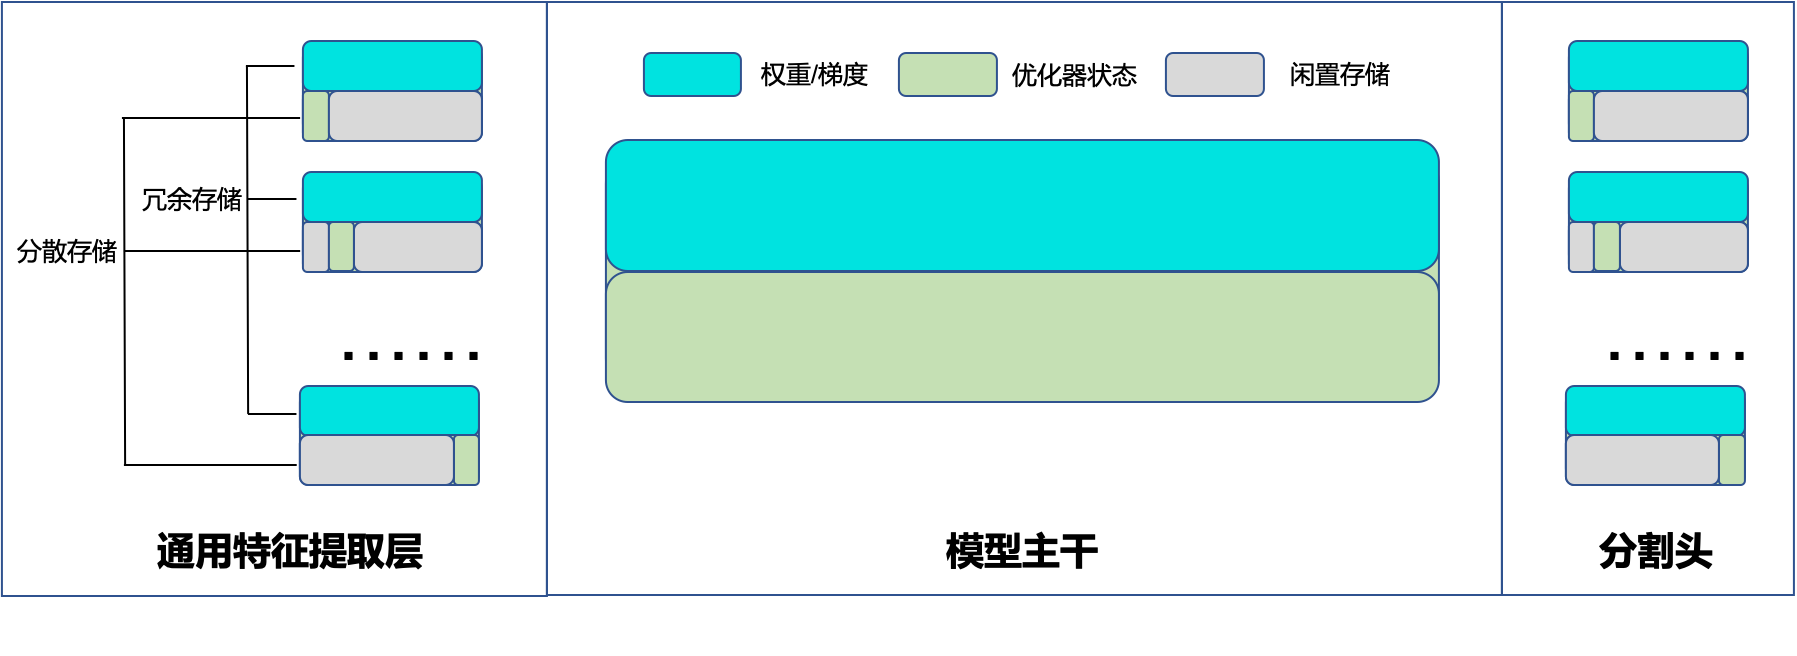
\includegraphics[width=0.75\textwidth]{figures/model_patition_method.png}
    \label{fig:diagram}
    \captionwithsource{MedFed联邦学习框架模型分割图}{}
\end{figure}


\subsection{模型参数更新策略}
\ensubsection{Model Parameter Update Strategy}



\subsection{动态批次组建}
\ensubsection{Dynamic Batching}
为了提升模型的训练速度,和减少数据中心模型的闲置时间,我们引入了动态批次组建的方法。具体来说,我们引入两个参数,全局批次大小$GBS$和局部批次大小$MBS$。
不同的医院客户端的计算能力、与数据中心的通信带宽和延迟都是不同的。因此,不同的医院客户端在给数据中心发送激活值的时候,发送的量和频率都是不同的。
在数据中心收到$MBS$个激活值之后,我们就会将这$MBS$个激活值组成一个批次,然后进行一次前向和反向传播。这一步需要的时间与数据中心分配给这个任务的算力
成正比,设这个时间为$t_{\text{calc}}$。同时,我们设置数据中心收到$MBS$个激活值的时间为$t_{\text{recv}}$。

我们进一步考虑了数据中心在处理这些批次时的效率问题。我们定义了一个效率比率$\eta$,
它是基于计算时间$t_{\text{calc}}$和接收时间$t_{\text{recv}}$的函数,用来衡量数据中心处理批次的效率。公式如下:
\begin{equation}
    \eta = \frac{t_{\text{calc}}}{t_{\text{recv}}}
\end{equation}

理想情况下,我们希望$\eta$接近于1,这意味着数据中心的计算能力与接收激活值的速度保持平衡。
这是因为,一个批次的处理时间由接收激活值的时间和前向反向传播中较长的一个决定。
当我们通过调节数据中心的算力,使得$\eta$接近于1时,我们的训练过程就如图3.2所示,可以看到,数据中心的计算能力和接收激活值的速度是保持平衡的。

\begin{figure}
    \centering
    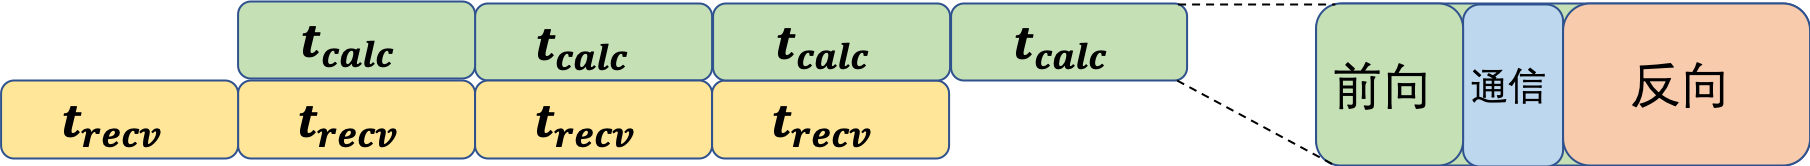
\includegraphics[width=0.75\textwidth]{figures/medfed_efficiency.png}
    \label{fig:diagram}
    \captionwithsource{MedFed联邦学习框架效率图}{}
\end{figure}


在这种情况下,我们可以计算的数据中心对于算力的浪费,
因为数据中心的优化器更新不需要通信,因此在耗时上总是更短的,设数据中心的优化器更新时间为$t_{\text{opt\_center}}$,医院客户端的优化器更新时间为$t_{\text{opt\_client}}$。
则数据中心对的有效率计算时间为:
\begin{equation}
    t_\text{efficiency} = \frac{\frac{GBS}{MBS} * t_{\text{calc}} + t_\text{opt\_center}}{\frac{GBS}{MBS} * t_{\text{calc}} + 1 * t_{\text{calc}} + t_{\text{opt\_client}}}
\end{equation}



\subsection{数据异构解决方案}
\ensubsection{Data Heterogeneity Solution}
第二个问题是尽可能消除非独立同分布数据对模型训练的影响。数据的异构性一直是联邦学习中的一个重要问题\supercite{DBLP:journals/corr/abs-2106-06843},因为不同的医院客户端的数据分布是不同的,如果不做任何处理,
这就会导致模型的训练效果很差。首先我们确保来自不同的数据分布的数据在一次训练中是均匀分布的(需要引用)。。。。。

\subsection{历史特征交换采样}
\ensubsection{Stable Feature Fusion}
其次根据我们所采用的实际的分割模型(存在一个教师模型,和一个学生模型,学生模型通过指数平均算法更新教师模型\supercite{DBLP:journals/corr/TarvainenV17})
也就是教师模型是更新的相对缓慢的,因此对同一个样本而言,输入到相邻训练步数的教师模型中,得到的特征是相似的,因此我们可以定义一个历史窗口,
这个历史窗口内的模型我们认为他们是有效的模型,但是距离当前时间点越远的模型,他的权重会越小,公式如下:
\begin{equation}
    \omega_{t} = \frac{1}{1 + \alpha(t_{\text{cur} - t})}
\end{equation}
其中$\omega_{t}$表示模型的权重,$t_{\text{cur}}$表示当前时间点,$t$表示模型的时间点,$\alpha$表示一个超参数,用来调整模型的权重。



\begin{figure}
    \centering
    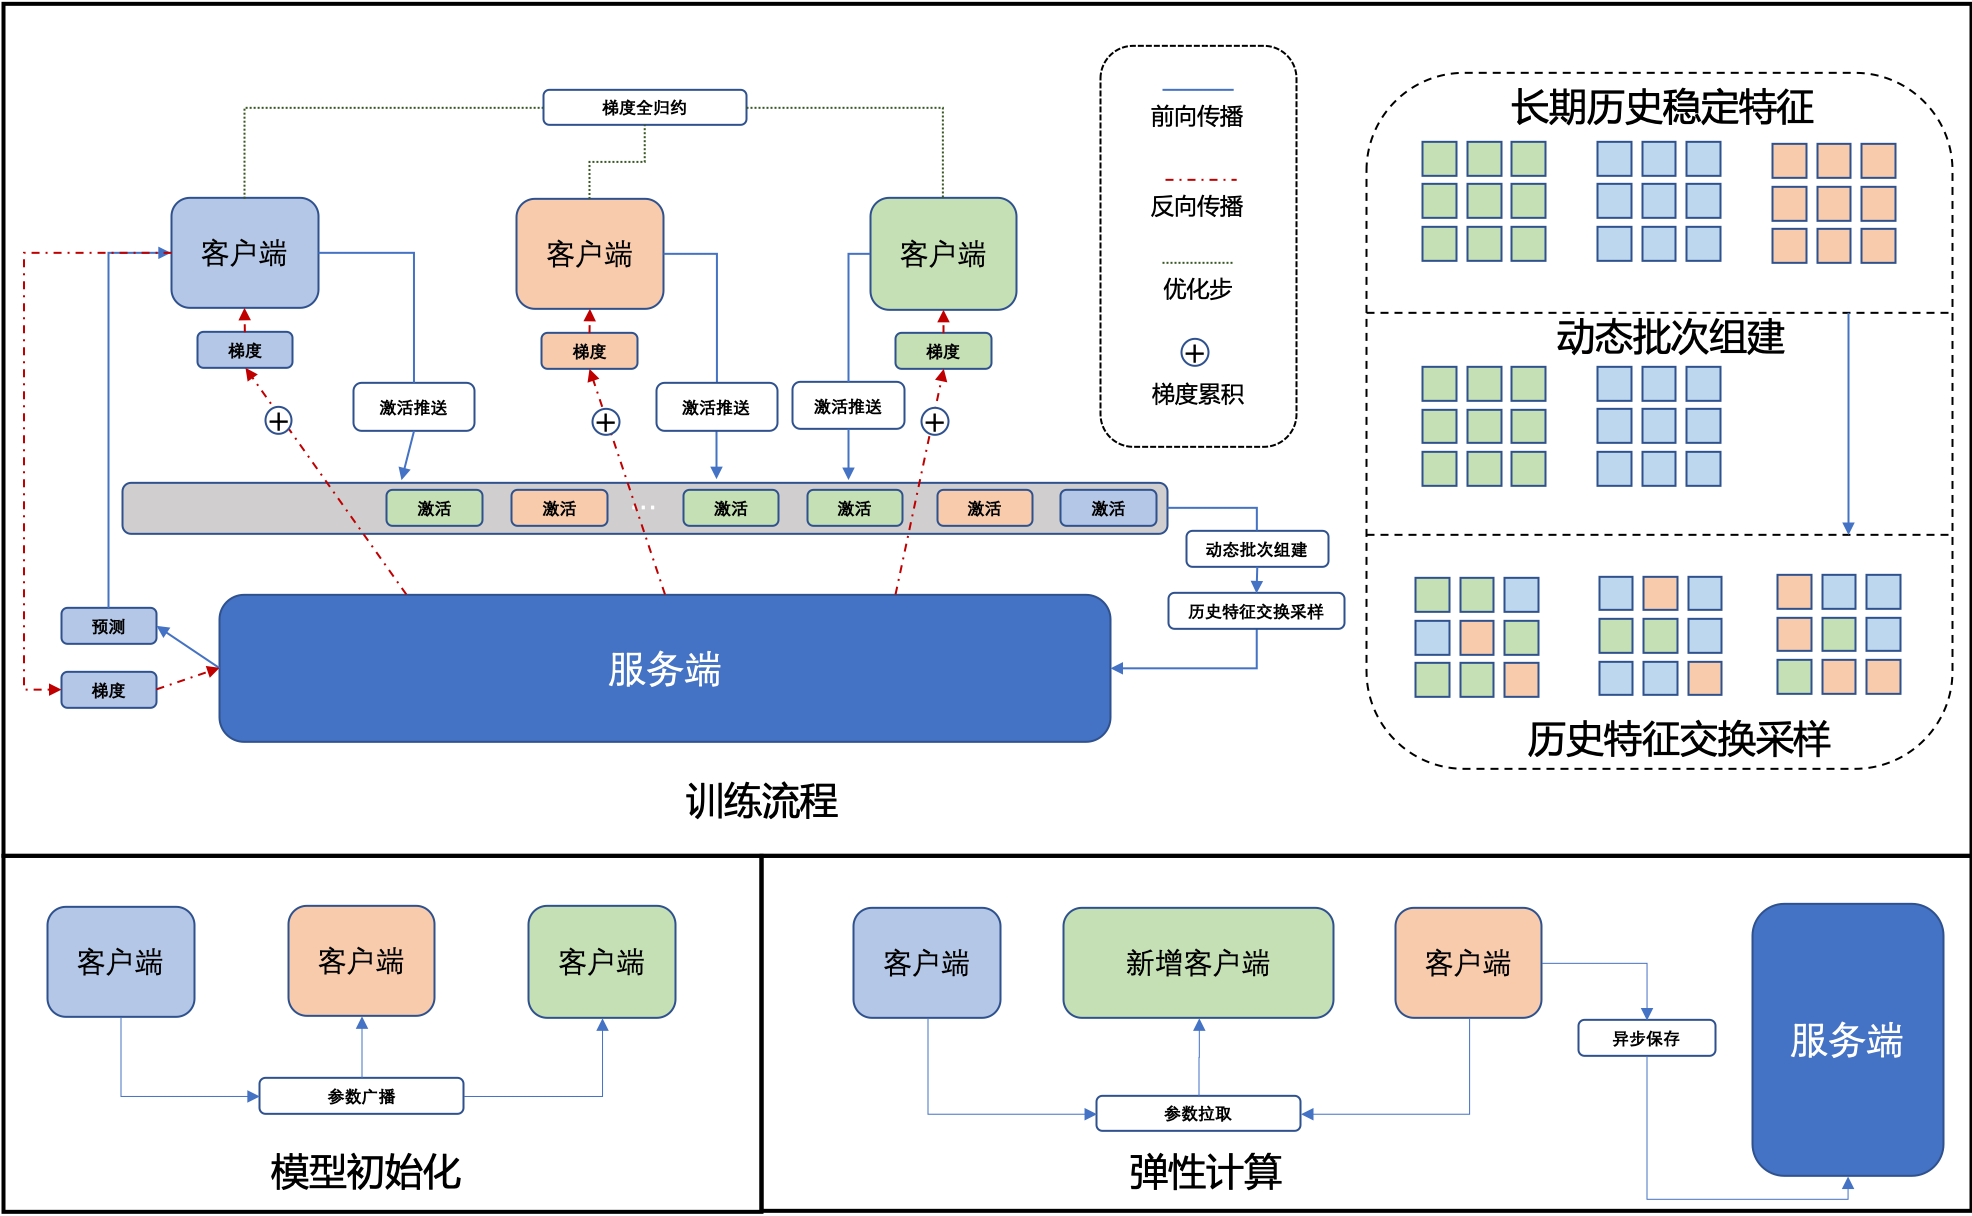
\includegraphics[width=0.75\textwidth]{figures/medfed_framework.png}
    \label{fig:diagram}
    \captionwithsource{MedFed联邦学习框架结构图}{}
\end{figure}

\section{实验设置}
\ensection{Experimental Settings}







% \adjustafterskip %调整章节与正文的间距。临时解决方案。总结、参考文献、附录、致谢和发表的论文都会受到影响。
\input{chapters/conclusion}

% 参考文献
\bibliography{reference/chapter1,reference/chapter3,reference/all.bib}

% 附录(章节编号重新计算,使用字母进行编号)
\appendix
\setappendixnumberformat

\input{chapters/appendix1}
\input{chapters/appendix2}

%%%%%%%%%%%%%%%%%%%%%%%%%%%%%%
%% 后置部分
%%%%%%%%%%%%%%%%%%%%%%%%%%%%%%
\backmatter

% 致谢
\input{chapters/acknowledgements}

% 发表文章目录
\input{chapters/publications}
\cleardoublepage

\end{document}
